\documentclass[output=paper]{langsci/langscibook} 
\author{Steffen Höder\affiliation{Christian-Albrechts-Universität zu Kiel}}
\title[Grammatical arealisms across the Danish-German border]
      {Grammatical arealisms across the Danish-German border from a constructional perspective}

\abstract{German and Danish share a long, complex, and multifaceted history of language contact. Besides other contact scenarios, societal as well as widespread individual multilingualism has characterized the linguistic situation in the territory of the former Duchy of Schleswig (i.e. the northern part of the federal state of Schleswig-Holstein in Germany as well as the southernmost part of Jutland in Denmark) from the Early Middle Ages until the present day. In structural terms, this contact scenario has resulted in a range of areal features that are shared by a number of Danish and German varieties spoken in the border region, while diverging markedly from other varieties of at least one of the languages. The aim of the present article is twofold: Firstly, it discusses selected grammatical arealisms found in dialectal and regiolectal varieties within the Danish-German contact zone (e.g. a \textsc{shall} future, the use of \textsc{and} words as infinitive markers in German varieties, and possessive linking pronouns in Danish dialects). Secondly, it attempts to demonstrate that such arealisms can be interpreted and, to some extent, explained within the framework of Diasystematic Construction Grammar (DCxG), a usage-based constructionist approach to language contact situations that is centred around the idea of language-unspecific constructions used in multilingual communities. Even though present-day speaker communities in the contact zone might not be equally bilingual as, say, their predecessors in the early 19th century, it is argued that the reconstruction of common constructions can help to better understand contact-related developments that led to the emergence of linguistic areality in the past.}

\IfFileExists{../localcommands.tex}{
  % add all extra packages you need to load to this file

\usepackage{tabularx,multicol}
\usepackage{url}
\urlstyle{same}

\usepackage{listings}
\lstset{basicstyle=\ttfamily,tabsize=2,breaklines=true}

\usepackage{langsci-optional}
\usepackage{langsci-lgr}
\usepackage{langsci-gb4e}
% \usepackage{langsci-plots}
\usepackage{pgfplots}

\usepackage{siunitx}
\sisetup{group-digits=false}

\usepackage{amssymb}% http://ctan.org/pkg/amssymb
\usepackage{pifont}% http://ctan.org/pkg/pifont
\newcommand{\cmark}{\ding{51}}%
\newcommand{\xmark}{\ding{55}}%
% \usepackage[disable]{todonotes}
\usepackage{todonotes}

  \newcommand*{\orcid}{}
\newcommand{\hoederN}{n̡} 
  %% hyphenation points for line breaks
%% Normally, automatic hyphenation in LaTeX is very good
%% If a word is mis-hyphenated, add it to this file
%%
%% add information to TeX file before \begin{document} with:
%% %% hyphenation points for line breaks
%% Normally, automatic hyphenation in LaTeX is very good
%% If a word is mis-hyphenated, add it to this file
%%
%% add information to TeX file before \begin{document} with:
%% %% hyphenation points for line breaks
%% Normally, automatic hyphenation in LaTeX is very good
%% If a word is mis-hyphenated, add it to this file
%%
%% add information to TeX file before \begin{document} with:
%% \include{localhyphenation}
\hyphenation{
affri-ca-te
affri-ca-tes 
}
\hyphenation{
affri-ca-te
affri-ca-tes 
}
\hyphenation{
affri-ca-te
affri-ca-tes 
} 
  \togglepaper[1]%%chapternumber
}{}

\begin{document}
\maketitle 


\section{Introduction}
\label{sec:hoeder:1}
\todo[inline]{check {\hoederN}}

German varieties have been in contact with Nordic languages throughout their history, involving a range of multifaceted contact scenarios. The majority of these scenarios fall into one of two (partially overlapping) categories:

\begin{enumerate}
	\item Northern German varieties (including both Low and High German) and Continental Scandinavian languages have been in long-term, intense contact from the Late Middle Ages onwards until (at least) the 19th century. Merchants from Northern Germany established trading routes to Scandinavia during the Hanseatic era, which not only resulted in a permanent presence of German-speaking people in Northern Europe (including large-scale migration by Germans into Scandinavian towns), but also marked the beginning of a centuries-long period that saw German as a culturally and economically prestigious, if not dominant language in Scandinavia. German has, as a consequence, influenced the Continental Scandinavian languages structurally in many ways, ranging from uncountable lexical and grammatical borrowings to the adoption of textual and stylistic norms (cf. \citealt{Braunmuller.2005}).

	\item In addition, German and Danish varieties have been in continuous contact since protohistoric times (which, for this area, means the Early Middle Ages) in what is now the Danish-German border region. Unlike other language contact areas, where rather clear-cut boundaries between different neighbouring languages have emerged over the centuries, there has usually been an areal overlap between Danish and German varieties within what is frequently called the Danish-German contact zone. This has led to different sociolinguistic scenarios for different historical periods, regions, and social groups, ranging from various types of diglossia (or, rather, polyglossia) and complex language shift scenarios to diverse settings of widespread individual and collective bi- or multilingualism (cf. \citealt{Fredsted.2009, Hoder.2019a}).
\end{enumerate}


On the whole, both scenarios have led to the emergence of areal features that are shared by both German and Nordic varieties, including lexical and phonological as well as grammatical \textit{arealisms}. While many of these arealisms are reflected in well-established and well-studied Germanisms in the Nordic standard varieties, others tend to remain underinvestigated, in particular those that only occur in non-standard varieties of either German or the Nordic languages. Such arealisms are the focus of the ongoing project \textit{Grammatical} \textit{Areality} \textit{in} \textit{the} \textit{Nordic} \textit{Countries} \textit{and} \textit{Northern} \textit{Germany} \textit{(GrammArNord)} at Kiel University (cf. \citealt{Hoder.2016a}).

The aim of the present article is twofold: Firstly, it discusses selected grammatical arealisms found in dialectal and regiolectal varieties within the Danish-German contact zone. Secondly, it attempts to demonstrate that such arealisms can be interpreted and, to some extent, explained within the framework of \textit{Diasystematic} \textit{Construction} \textit{Grammar} (\citealt{Hoder.2012, Hoder.2014, Hoder.2018}), a usage-based constructionist approach to language contact situations that is centred around the idea of language-unspecific constructions used in multilingual communities. Even though present-day speaker communities in the contact zone might not be equally bilingual as, say, their predecessors in the early 19th century, it is argued that the \textit{reconstruction} \textit{of} \textit{common} \textit{constructions} can help to better understand contact-related developments that led to the \textit{emergence} \textit{of} \textit{linguistic} \textit{areality} in the past.

The article is structured as follows: \sectref{sec:hoeder:2} gives a brief outline of the history (linguistic and otherwise) of the Danish-German contact zone, followed by a sketch of Diasystematic Construction Grammar (\sectref{sec:hoeder:3}), which also includes a discussion of major types of contact-related change from a diasystematic point of view. Against this background, five selected areal features are then discussed in detail in the following section (\sectref{sec:hoeder:4}). The final section provides concluding remarks (\sectref{sec:hoeder:5}).


%\section{The Danish-German contact zone}
\label{sec:hoeder:2}

Nordic and West Germanic varieties have been in continuous contact on the Cimbrian Peninsula (comprising the mainland of today’s Kingdom of Denmark and the federal state of Schleswig-Holstein within today’s Federal Republic of Germany) for more than a thousand years. By the end of the first millennium CE, the southern part of the peninsula was inhabited by speakers of four recognisably different language groups:

 \begin{enumerate}
	\item Saxons, settling in the south of the area, speaking Old Saxon, a West Germanic variety and the predecessor of Modern Low German;
	\item Jutes in the northern part of the region, speaking Old East Nordic varieties that later evolved into the (South) Jutlandic branch of Danish dialects;
	\item Frisians on the North Sea islands and along the coast of today’s North Frisia, whose language developed into distinct North Frisian dialects;
	\item Obotrites in the easternmost parts of Holstein, speaking varieties of Polabian belonging to the Lechitic branch of West Slavic.
	\end{enumerate}

Subsequent Germanisation of the Slavic-speaking population from the 12th century onwards resulted in a tripartite distribution of the regional languages that, in a way, still holds today, with Danish in the north, German in the south, and Frisian in the west.

While the contact linguistic macro-scenario has thus remained stable for more than a millennium, the actual \textit{ecologies}, to use \citegen{Haugen.1971} concept (cf. \citealt{Eliasson.2013}) – i.e. the social settings in which the languages have actually been used by their speaker communities – have changed frequently, often rather dramatically, and in quite complex ways over the centuries. The region’s linguistic history is inextricably intertwined with its sociocultural and (at times rather labyrinthian) political development.

For most of its history, the peninsula was mainly divided politically into three territories (cf. \figref{fig:hoeder:1}):


 \begin{enumerate}
	\item Northern Jutland (an integral part of the Danish realm), roughly north of the river Kongeå, flowing into the North Sea near Ribe;

	\item the Duchy of Schleswig (a Danish fief) between the rivers Kongeå and Eider, flowing into the North Sea south of Tönning in North Frisia;

 \item the Duchy of Holstein (a state within the Holy Roman Empire until 1806, later within the German Confederation) between the rivers Eider and Elbe.\footnote{This is a much simplified representation – in reality, the division was not always that neat. For one thing, numerous smaller polities existed in different parts of the southern region as well, all parts of the Holy Roman Empire and its successors, including the Duchy of Saxe-Lauenburg, the Republic of Dithmarschen, the Prince-Bishopric of Lübeck, and the Free and Hanseatic Cities of Lübeck and Hamburg. Also, the Duchy of Holstein was subdivided into different (but partly jointly ruled) sub-duchies during the Late Middle Ages and Early Modern Times. Finally, parts of the territory between the rivers Kongeå and Eider were ruled as enclaves of Denmark proper rather than as parts of the Duchy of Schleswig.}
	\end{enumerate}

\begin{figure}
%%please move the includegraphics inside the {figure} environment
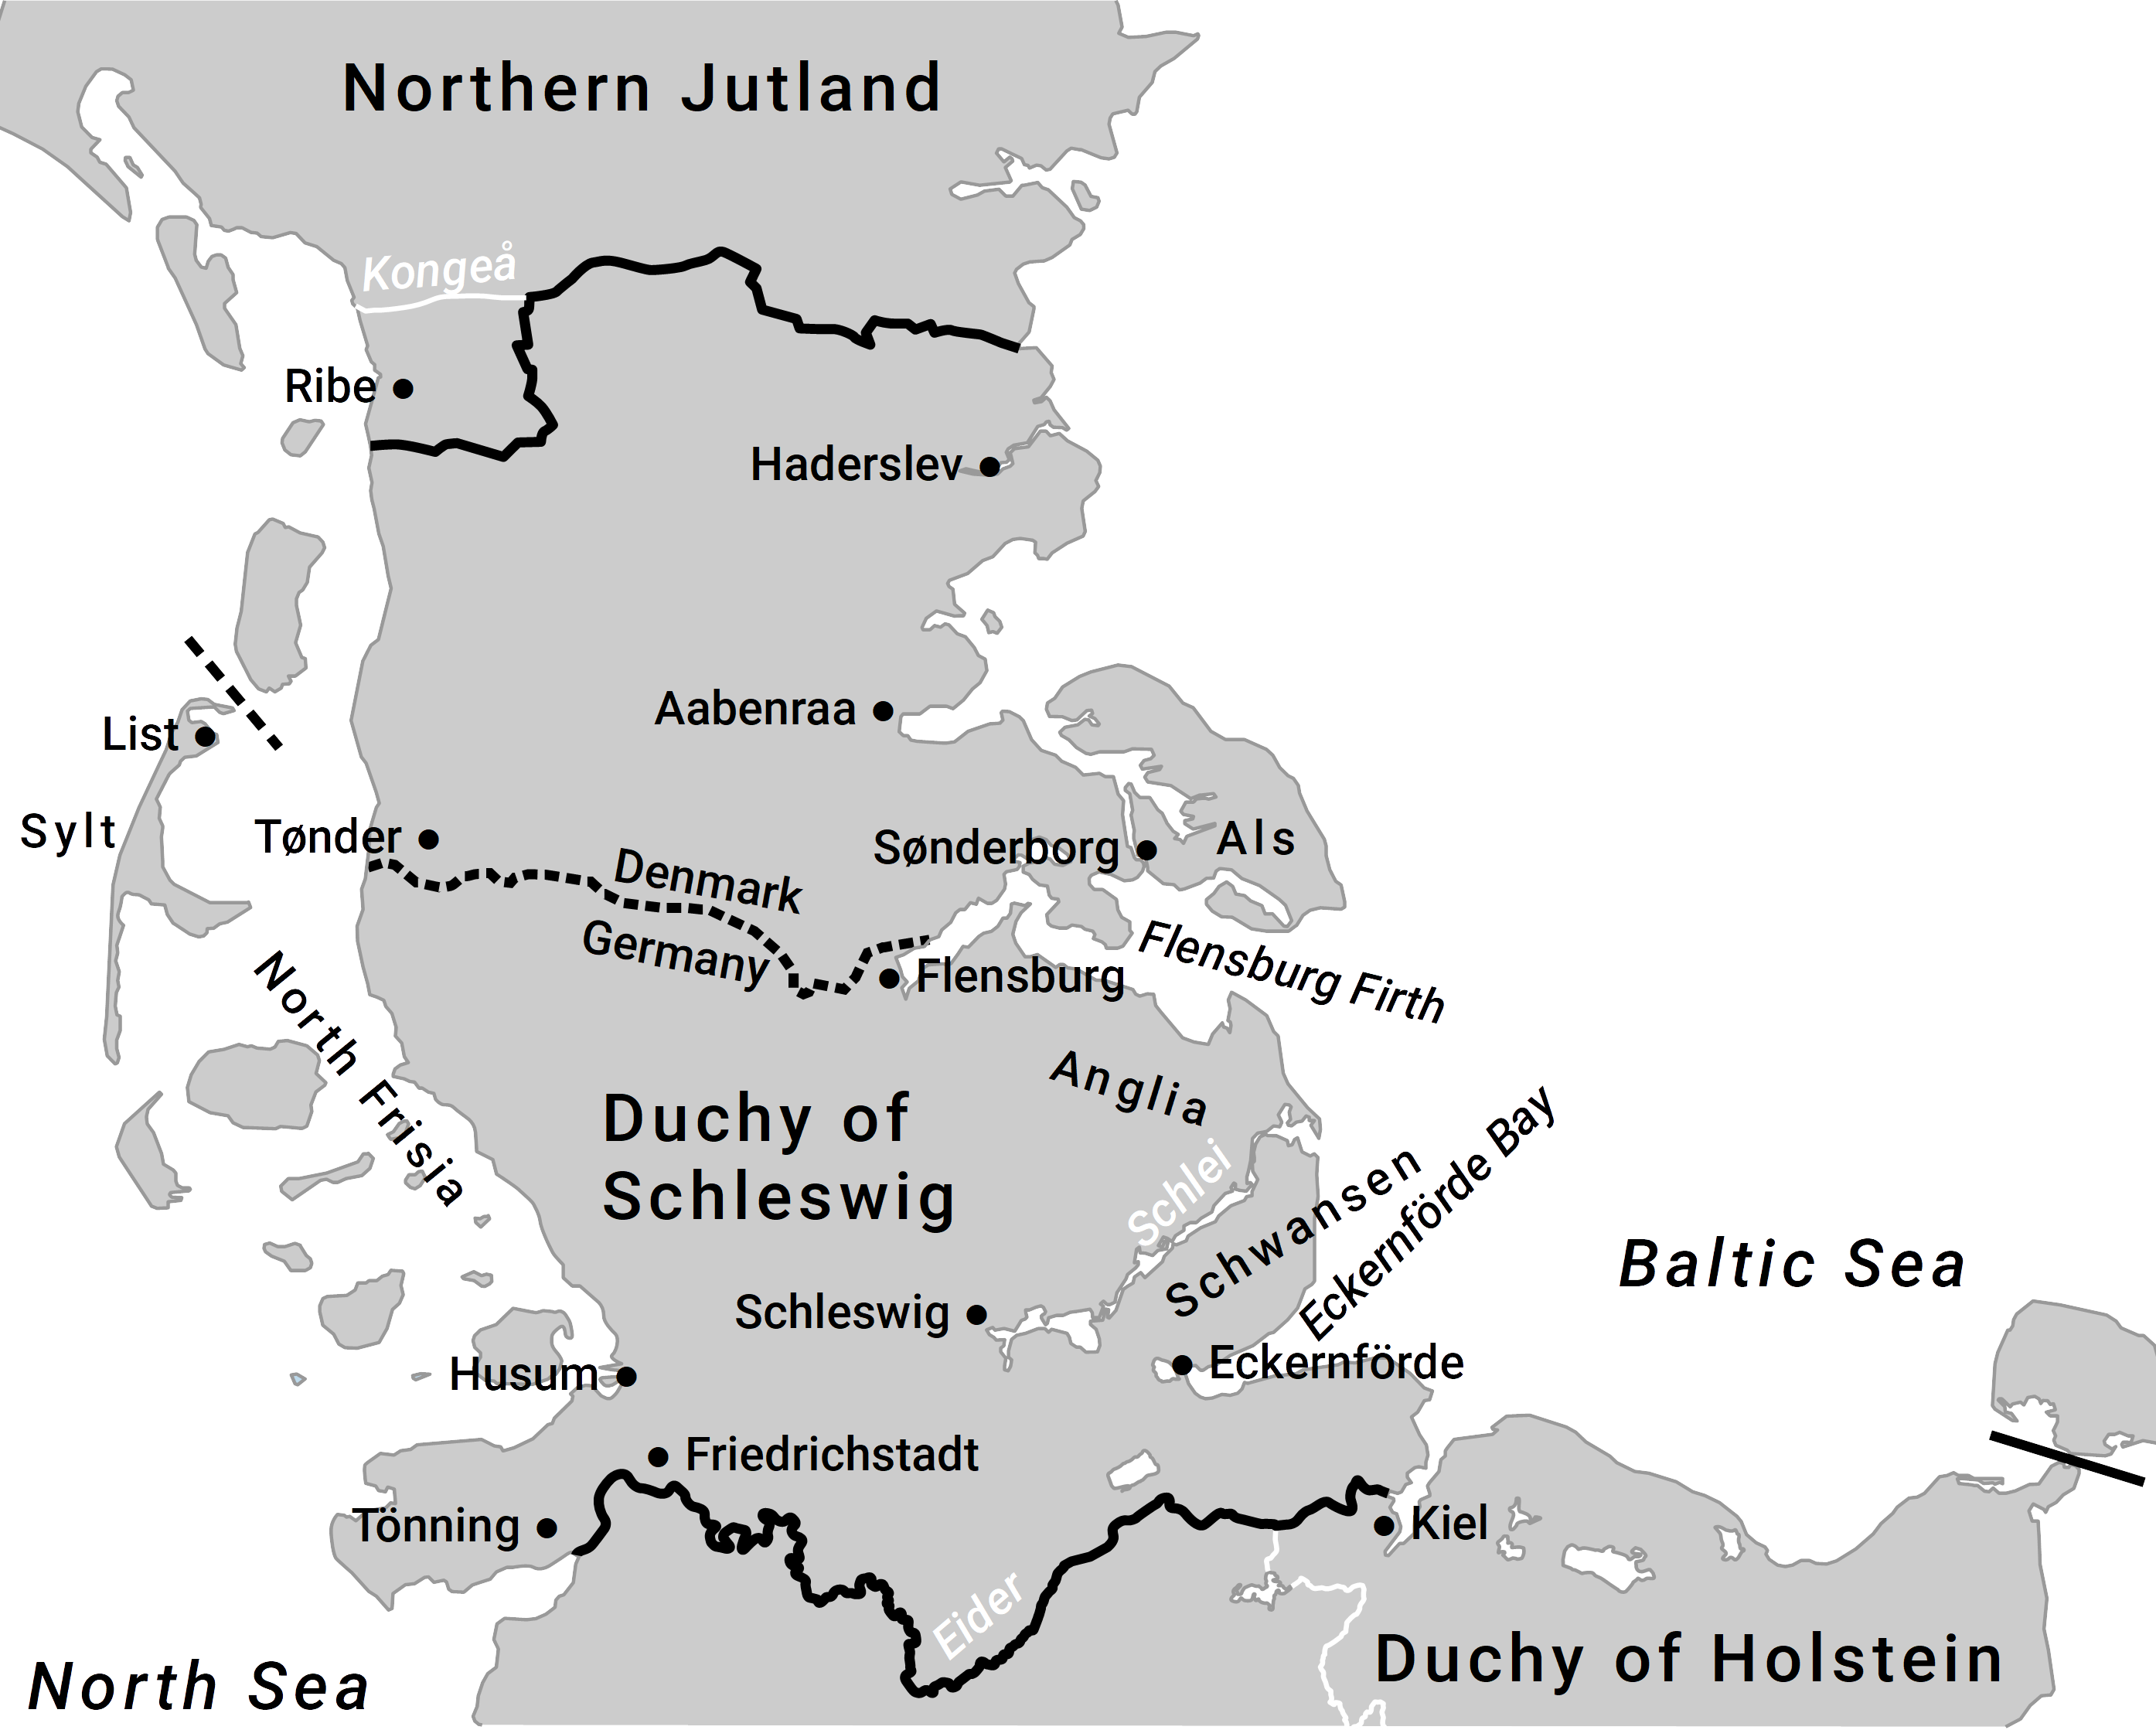
\includegraphics[width=0.8\textwidth]{figures/hoeder-map.png}
\caption{The Duchy of Schleswig (modified work, CC-BY-SA-3.0-DE, Steffen Höder. Original source: commons.wikimedia.org/wiki/File:Karte\_Deutsch-D\%C3\%A4nischer\_Krieg.svg by NordNordWest/Wikipedia)}\label{fig:hoeder:1}
\end{figure}

From the 15th until the 19th century, the duchies constituted semi-autonomous polities under Danish suzerainty, whose degree of political autonomy varied across historical periods; the Danish monarchs usually ruled both duchies either personally (by means of a personal union between the duchies and the kingdom) or indirectly (through dependent dukes).

During the heyday of nationalism in the 19th century, tensions arose between Denmark and the German Confederation over the territorial affiliation of the duchies. Denmark eventually lost their territory as a result of the Second Schleswig War in 1864, and Schleswig and Holstein were annexed by Prussia in 1866 and subsequently incorporated into the German Empire in 1871. After the First World War, two internationally monitored plebiscites in 1920 resulted in a partition of the former Duchy of Schleswig into a Danish and a German part, separated by a new border that has remained in place ever since. This partition, in turn, has resulted in the emergence of \textit{national} \textit{minorities} on both sides of the border, consisting of people that, for some reason, identify as German or Danish, respectively, while being citizens and inhabitants of the other country.\footnote{In everyday parlance, the northern part of the former Duchy is usually referred to as Southern Jutland (Danish \textit{Sønderjylland}, German \textit{Südjütland}), and the southern part is normally called Schleswig (Danish \textit{Slesvig}, German \textit{[Landesteil]} \textit{Schleswig}). In specific contexts – in particular when the national minorities are concerned – the northern and southern parts are referred to as North Schleswig (Danish \textit{Nordslesvig}, German \textit{Nordschleswig}) and South Schleswig (Danish \textit{Sydslesvig}, German \textit{Südschleswig}), respectively.} Both minorities are protected by an extensive framework of diplomatic, legal, and political measures at different levels (regional, national, supra-, and international), one of the earliest and most important steps being the 1955 Bonn-Copenhagen Declarations in which the governments of Denmark and West Germany granted concurrent rights to both minorities. Moreover, the minorities maintain their own institutions (e.g. pre-schools, schools, churches, and cultural as well as political organisations). There are no official criteria for minority membership (in fact, applying such criteria would be illegal in both countries), but there is a range of \textit{de} \textit{facto} criteria such as, most prominently, enrolment in minority schools.

Danish and German varieties have always coexisted territorially in the Duchy of Schleswig, with shifting types of polyglossic distributions in some parts of the region \citep{Winge.2004}. This is why the area is frequently described as a \textit{contact} \textit{zone} (as opposed to a language boundary, which would imply a possibility to draw a clear-cut line between a Danish-speaking and a German-speaking area). In addition, North Frisian dialects have been in continuous (but declining) use in North Frisia up to the present day, including the North Frisian Islands and a coastal strip on the mainland. (Frisian will, however, be largely excluded from the following discussion that instead focuses on Danish and German.) Until about 1800, Danish was used in everyday communication in rural areas north of a line between the towns of Friedrichstadt in North Frisia and Eckernförde on the east coast, whereas German was used south of that line. In the towns and among nobility and merchants, however, as well as in the domains of law and administration, German varieties – including Low and High German – were used predominantly by about 1500. The languages used in church and in school differed between ecclesiastical subdivisions such as dioceses, with Danish dominating north of Flensburg and German in the south (\citealt{Fredsted.2009}: 2–7). Functional and regional differentiation between languages and varieties notwithstanding, the major part of the Duchy of Schleswig can be appropriately described as a \textit{transnational} \textit{multilingual} \textit{communicative} \textit{space} until, say, 1800. Language choice was largely determined by pragmatic factors rather than national or ethnic affiliation, and multilingualism was, in some form and to some extent at least, the rule rather than the exception both at the collective and at the individual level (\citealt{Hoder.2019}: 56–58).\footnote{There is also ample metalinguistic evidence for the ubiquity of multilingual practices from early on; for example, the Danish scholar Christiern Pedersen (1531, \textit{Dauidz} \textit{psaltere}, fol. Tviijr, as quoted by \citealt[162]{Skautrup.1947}), characterises the Danish variety spoken in Flensburg as incomprehensible to speakers from Denmark proper because of the amount of German transferences.}

The 19th century, however, saw an accelerating language shift from Danish dialects to German varieties in everyday domains in rural areas in the south \citep[59]{Hoder.2019}. Although there were concerted political efforts from both the Danish side and, after 1864, the Prussian side as well to strengthen the respective national languages and suppress the use of the minority languages, the shift towards German is rather due to the higher societal prestige of German (as, among other things, the language of the social, economic, and cultural elites) and its wider functional and geographic range. The shift began in the eastern regions and proceeded westward. While the Danish-speaking area in 1600 had included the Schwansen peninsula (between the Schlei, a firth east of Schleswig, and Eckernförde Bay), this region had shifted to German by about 1780. By 1850, the shift was completed in Anglia (between the Schlei and the Flensburg Firth). \citep[3--6]{Wenker.2013}, in his map and commentary, reported the ongoing shift and noted that young people no longer used Danish in north-western Central Schleswig around 1880. One consequence of this successive shift to German varieties is the emergence of Low German dialects (Schleswig Low German) used in previously Danish-dominant communities.

In the 20th century, in turn, many speakers \textit{shifted} \textit{from} \textit{dialectal} \textit{to} \textit{more} \textit{standard-like} \textit{regional} \textit{varieties} of German and Danish, respectively, in domains of everyday communication, resulting in declining dialect use and often even dialect loss \citep[62]{Hoder.2019}. In the latter case, the process also entailed the replacement of a diglossic distribution of the dialects and the respective standard varieties with \textit{diaglossic} \textit{repertoires} \citep{Auer.2011} that comprise near-standard varieties as well as more standard-divergent regiolectal varieties, in particular in South Schleswig (\citealt{Hoder.2011}; \citeyear{Hoder.2019}: 65--71), whereas speakers in North Schleswig maintain diglossia to a higher extent.

The resulting situation is further complexified by the emergence of \textit{minority} \textit{varieties} used by the national minorities on both sides of the border (North Schleswig German, Danish \textit{nordslesvigtysk}, German \textit{Nordschleswigdeutsch}, and South Schleswig Danish, Danish \textit{sydslesvigdansk}, German \textit{Südschleswigdänisch}). These varieties show virtually no traces of the traditional dialects of the minority languages, but are instead heavily influenced by contact with the standard varieties of the national languages in the respective countries. The main reason for this is institutional: While speaking the minority language – let alone being an L1 speaker – is not necessary for minority membership, the institutions conduct their official business in the minority languages; in particular, they are the primary languages of instruction in minority schools. As a consequence, active participation in minority institutions requires some form of linguistic competence, and the institutions are the most important locus of minority language acquisition. Virtually all minority language speakers are bilingual, and most are L1 speakers of the respective majority language, whereas the minority language is acquired as a second L1 or as an early L2, during pre-school and school education (\citealt{Kuhl.2015}: 246–247).

\tabref{tab:hoeder:1} summarises the varieties of Danish and German that are used in the former Duchy of Schleswig today (in addition to North Frisian dialects, Romani, Danish Sign Language, German Sign Language, and post-1950 migrant languages).

\begin{table}
\begin{tabularx}{0.95\textwidth}{p{1.7cm} p{4.cm} p{4.5cm}}
\lsptoprule
 variety & Danish & German\\
 \hline
standard & Standard Danish & Standard (High) German\\
regiolectal & Jutlandic Danish & North High German\footnote{The term \textit{North} \textit{High} \textit{German} is preferred over alternative terms such as \textit{Northern} \textit{Standard} \textit{German} or simply \textit{Northern} \textit{German} because it emphasises the dialectologically relevant difference between High German varieties and Low German varieties. Socio-politically speaking, Low German and High German are usually considered to be different languages, with Low German lacking a standard variety of its own.}\\
local & local varieties of Jutlandic Danish & local varieties of North High German\\
dialectal & (local) South Jutlandic & (local) Schleswig Low German\\
minority & South Schleswig Danish & North Schleswig German\\
\lspbottomrule
\end{tabularx}
	\caption{Danish and German in North and South Schleswig.}
	\label{tab:hoeder:1}
\end{table}

It is no surprise that, after almost a millennium of rather intense language contact, the languages spoken in the area have become increasingly similar in structural terms. This development has not escaped the attention of linguists either. Among the contact-induced innovations that have been described in the dialectological and contact linguistic literature are both lexical items (e.g. South Jutlandic and local Jutlandic Danish \textit{mojn} ‘hello; bye’ < Low German, North High German \textit{moin} ‘hello’; the original etymology is unclear; \citealt{Pedersen.1995}) and structural patterns (such as the de-additive infinitive, see \sectref{sec:hoeder:4.3}). However, they are usually analysed in \textit{linguocentric} \textit{terms}, i.e. as borrowings from one language into another, and only rarely viewed from an \textit{areal} \textit{perspective}, i.e. with a focus on structures that are shared across languages within a specific area in communicative space, in particular when this area extends beyond the border region in a narrow sense (such as with de-demonstrative phoric pronouns, an areal feature that is found in all of the Scandinavian languages as well as in German varieties north of the Elbe; \citealt{Hoder.2016a}: 121–124).


% \section{Grammatical arealisms from a constructional perspective} %3
\label{sec:hoeder:3}

There is a cognitive dimension to the increasing similarity of neighbouring languages that underlies the emergence of grammatical arealisms: In the contact zone, \textit{individual} \textit{bi-} \textit{or} \textit{multilingualism} has, at least, been widespread at some point in history. In usage-based or cognitive terms, the fact that stable, intense, long-term contact typically increases (or inhibits a decrease in) structural similarity between the varieties involved (cf. \citealt{Matras.2010}) reflects the more general pattern that multilingual speakers prefer, evolve, and retain structures that are applicable in more than one of their languages, i.e. structures that are shared by several varieties. This is in line with the view held by modern contact linguistics (e.g. \citealt{Matras.2020}: 336) that multilinguals do not store or process linguistic elements separately for each of their languages, but rather organise their linguistic knowledge in its entirety into a common repertoire from which they choose the appropriate structures in a given communicative situation.

Diasystematic Construction Grammar (DCxG; \citealt{Hoder.2012, Hoder.2014, Hoder.2018, Hoder.2019b}; for an extensive survey, see \citealt{Hoder.2018}) is, basically, a somewhat formalised model of this view in terms of a usage-based Construction Grammar approach to language contact situations.\footnote{Construction Grammar can be understood as a family of grammatical theories that share the idea of the construction as the central unit of language structure, defined as form-meaning pairs (for an overview, cf. \citealt{Hoffmann.2013}; \citealt{Hilpert.2019}). Proponents of usage-based Construction Grammar (for an overview, cf. \citealt{Diessel.2019}) emphasise the cognitive side of language and thus consider constructions as (cognitively realistic) representations of speakers’ linguistic knowledge.} DCxG embraces the view put forward by, among others, \citet[18]{Goldberg.2006} that speakers’ linguistic knowledge in its entirety can be captured by a \textit{constructicon}, i.e. a set of constructions connected by interconstructional links – which implies that the language-specificity of linguistic elements must be represented constructionally as well. In DCxG, language-specificity is conceptualised as a property of individual constructions, i.e. as part of a construction’s pragmatic meaning, within an inherently \textit{multilingual} \textit{constructicon}. The rationale behind this conceptualisation is that multilingual speakers use different languages for different purposes (\citeauthor{Grosjean.2008}'s \citeyear{Grosjean.2008}: 22--31 ‘Complementarity Principle’), i.e. language choice is functional in that it conventionally marks the current context as belonging to a specific set of communicative settings.

For example, a bilingual member of the Danish minority in Germany will typically use Danish words such as \textit{by} ‘town’ in institutional minority contexts, but German words such as \textit{Stadt} ‘town’ when talking to colleagues and neighbours that do not belong to the minority; this is not merely an individual habit, but a communicative convention shared by the whole bilingual community. These are examples of language-specific constructions, or, in DCxG terminology, \textit{idioconstructions}; they can be formalised as, say, {[}\textit{by} ‘town’ $\langle$C\textsubscript{minority institutions}$\rangle${]} and {[}\textit{Stadt} ‘town’ $\langle$CC\textsubscript{everyday life}$\rangle${]}. The label C\textit{\textsubscript{x}} specifies the set of communicative settings that the construction marks; a common shorthand notation is the use of C\textit{\textsubscript{glottonym}} (e.g. $\langle$CC\textsubscript{Danish}$\rangle$), which suggests that the construction is used in a set of contexts (whatever they are) that are conventionally associated with language X in a given community.

However, DCxG emphasises that, since ‘language’ is a sociolinguistic (or, if not even that, a metalinguistic) label rather than an \textit{a} \textit{priori} cognitive category, there is no need for \textit{all} constructions to be language-specific. For example, a member of the German minority in Denmark cannot use \textit{mojn/moin} ‘hello’ to mark the current context as belonging to some specific set of communicative settings, since this lexical element is shared by all of the dialectal and regional varieties in her repertoire (e.g. local Jutlandic Danish, South Jutlandic, North High German). This is an example of a language-unspecific \textit{diaconstruction}, i.e. a construction that does not carry pragmatic meaning of the$\langle$C\textsubscript{x}$\rangle$ type.

As constructions in general, diaconstructions come in different degrees of schematicity, ranging from fully filled constructions (without any open slots) such as free lexemes (e.g. \textit{mojn/moin}) via partially filled constructions to fully schematic ones. Standard Danish, for example, has a fully schematic clausal construction {[}\textsc{v}\textsubscript{fin}\textsuperscript{1} \textsc{subj} … $\langle$polar question$\rangle${]}, i.e. a syntactic pattern that consists of a clause-initial finite verb followed by a subject and, optionally, other elements, and functions as a polar question marker.\footnote{The following notational conventions apply throughout this contribution: \textit{italics} = lexical form; \textsc{small} \textsc{capitals} = schematic form; \textsc{italic} \textsc{small} \textsc{capitals} = paradigmatic form; ‘ ’ = lexical meaning (indicated by approximate translation); {$\langle$} {$\rangle$} grammatical/pragmatic meaning (indicated by approximate description); … (ellipsis) = other (compulsory or optional) components of a construction (left out in the description); X\textsubscript{property:value} = an element X with a specific property with a specific value; X\textsubscript{property:α} = a variable value of a property; X\textsuperscript{number} = relative position of an element X within a construction; X~Y = elements X and Y are adjacent to each other; X,~Y = elements X and Y are components of the construction (but do not necessarily occur in that order or adjacent to each other).} However, the same construction – {originally a common Germanic feature –} is also used in non-standard Danish and even in German varieties spoken in Schleswig, such as Jutlandic Danish, South Jutlandic dialect, Schleswig Low German, North High German, and Standard German, as illustrated in \REF{ex:hoeder:1}:


 
\ea\label{ex:hoeder:1}
	\ea \label{ex:hoeder:1a}
	Standard Danish, Jutlandic Danish\\
	\gll \textbf{Kunne} \textbf{I} hør-e mig?\\
     	can.\textsc{prt} \textsc{2pl.nom} hear-\textsc{inf} 1\textsc{sg.obl}\\
	
	\ex\label{ex:hoeder:1b}
		South Jutlandic dialect\\
		\gll \textbf{Ku} \textbf{I} hye mæ?\\
     	can.\textsc{prt} \textsc{2pl.nom} hear.\textsc{inf} 1\textsc{sg.obl}\\
     	
	\ex\label{ex:hoeder:1c}
	 Schleswig Low German\\
	\gll \textbf{Kunn-en} \textbf{ji} mi hör-en?\\
     can.\textsc{prt-pl} 2\textsc{pl.nom} 1\textsc{sg.obl} hear\textsc{{}-inf}\\
     
	\ex\label{ex:hoeder:1d}
	Standard German, North High German\\
	\gll \textbf{Konn-te-t} \textbf{ihr} mich hör-en?\\
     can{\textbackslash}\textsc{prt-prt-}2\textsc{pl} 2\textsc{pl.nom} 1\textsc{sg.acc} hear-\textsc{inf}\\
	\glt `could you hear me?'
\z
\z

While there are numerous grammatical differences between the utterances in the different languages and varieties (as indicated by the glossing) and the lexical filling, of course, is language-specific, a speaker that has these varieties in her repertoire can use the same Verb-Initial Polar Question Construction in any communicative context. For multilingual speakers, then, this construction qualifies as a schematic diaconstruction, a syntactic pattern that can be used across languages.

Whether there is a diaconstruction that is shared, as it were, by different languages used by the same speaker community, or whether there are different (but parallel) constructions in each variety is not only a matter of descriptive preference or elegance. Diaconstructions are cognitively more economic, since using the same construction across languages simplifies the overall organisation of multilingual speakers’ linguistic knowledge. DCxG predicts, among other things, that multilinguals have a preference for diaconstructions over idioconstructions (as compared to, for instance, monolingual speakers of the languages involved). They will also use diaconstructions productively, resulting in diasystematically anchored innovations, i.e. forms that are non-canonical, but perfectly acceptable for members of the multilingual community (while they may be incomprehensible to monolingual outsiders; \citealt{Hoder.2018}: 59; \citeyear{Hoder.2019b}: 347--348). In the long run, such innovations may be entrenched and conventionalised, which then results in language change.

Arealisms typically come into being through common inheritance in neighbouring languages (as with verb-initial polar questions) or through contact-induced convergence. From a DCxG perspective, a high amount of arealisms in a given region corresponds to a high \textit{degree} \textit{of} \textit{diasystematicity}, defined as \textit{the} \textit{proportion} \textit{of} \textit{diaconstructions} in \textit{the} \textit{multilingual} \textit{constructicon} that encompasses the respective languages. The degree of diasystematicity is influenced by various factors:

\begin{enumerate}
 \item First of all, it is obvious that the languages and varieties in many contact areas, such as the Danish-German contact zone, are genetically closely related and, unsurprisingly, structurally rather similar; their overall degree of diasystematicity is high from the outset, i.e. many of their structures can be stored and processed as diaconstructions, in particular schematic ones such as the Verb-Initial Polar Question Construction.

 \item Irrespectively of such pre-existing similarities, intense language contact will result in an increase in diasystematicity. It has often been observed that, given enough time, languages in contact will approximate (and potentially reach) a form of structural isomorphism between larger portions of the language systems, variously described in the literature as, for example, “exact structural equivalence" (\citealt{Heine.2005}: 179--180), “word-for-word and morpheme-per-morpheme intertranslatability" \citep[28]{Aikhenvald.2006}, or “construction-per-construction intertranslatability" \citep[149]{Hoder.2014}. The key mechanism behind such convergence processes, constructionally speaking, is what has been called \textit{pro-diasystematic} \textit{change} (\citealt{Hoder.2018}: 59--62), basically a type of pragmatic bleaching in which an idioconstruction gradually loses its pragmatic restriction to a (language-)specific set of communicative settings until it is considered acceptable in a wider range of contexts, i.e. as a diaconstruction. Pro-diasystematic change, then, is essentially an economic process, a simplification of the multilingual constructicon (for examples, see \sectref{sec:hoeder:4.4}--\sectref{sec:hoeder:4.6}).

 \item Pro-diasystematic change may also entail mechanisms of constructional reorganisation that facilitate diaconstructional processing in more sophisticated ways. For example, existing idioconstructions or interconstructional links can be modified so as to increase the degree of diasystematicity in a specific part of the constructicon (\textit{diaconstructionalisation}; see \sectref{sec:hoeder:4.3} for an example).

 \item Finally, arealisms may reflect \textit{diasystematic} \textit{stability:} existing diaconstructions in regional varieties fail to undergo language-specific changes that are going on in other regions where one of the contact languages is spoken (cf. \citealt{KühlBraunmüller2014}; see \sectref{sec:hoeder:4.2} for a potential instance).
 
 \end{enumerate}



From a cognitive view, the locus of language contact is “the language processing apparatus of the individual multilingual speaker and the employment of this apparatus in communicative interaction' \citep[3]{Matras.2020}. Once established, however, contact-induced arealisms continue to exist even when speakers no longer are multilingual, and areal patterns often reflect historical contact situations rather than present-day multilingualism. Yet, a usage-based framework such as DCxG can still be employed as a descriptive tool for the analysis of grammatical arealisms that also has explanatory power, since areal features can be described in terms of \textit{reconstructed} \textit{diaconstructions} for the multilingual communities in which they supposedly originated (cf. \citeauthor{Holzl.2018}’s \citeyear{Holzl.2018} notion of \textit{constructionalisation} \textit{areas}). As with all types of linguistic reconstruction, however, caution is advised, since a fuller analysis (e.g. using a historical sociolinguistic approach) would require detailed information on the respective ecologies of these communities, including information on chronology and sociolinguistic settings – which, unfortunately, are usually not known in detail.


% \section{Analysis of selected areal features}
 \label{sec:hoeder:4}


 \subsection{Feature catalogue}
 \label{sec:hoeder:4.1}

The following sections contain brief analyses of five grammatical arealisms (see \tabref{tab:hoeder:2}) from the Danish-German contact zone, illustrating different types of diasystematic innovations. None of these features are totally innovative in the sense that they do not occur anywhere outside the contact zone. Rather, they reflect bilingual innovations that facilitate an areal spread of originally Danish (or, more generally, Nordic) features into German varieties (features 1--3) or vice versa (features 4--5). Also, almost all of the features have been described in earlier research (features 1--4), but usually without much focus on cognitive aspects or even an areal perspective. Among those, some of the features (1--2) are fairly well-known as regional markers among the population, whereas others are primarily known from the dialectological literature (features 3--4). Finally, one feature \REF{ex:hoeder:5} has not been dealt with extensively in prior research.

\begin{table}
\begin{tabularx}{0.7\textwidth}{p{0.5cm}X}
\lsptoprule
{[1]} & {De-Obligative Future Construction}\\
{[2]} & {De-Additive Infinitive Construction}\\
{[3]} & {Animacy-Gender-Sex Pronominalisation Constructions}\\
{[4]} & {Possessive Linking Pronoun Construction}\\
{[5]} & Dative External Possessor Constructions\\
\lspbottomrule
\end{tabularx}
\caption{Grammatical arealisms in the Danish-German contact zone (selection).}
\label{tab:hoeder:2}
\end{table}




\subsection{De-Obligative Future Construction}
\label{sec:hoeder:4.2}

German varieties in the contact zone have a standard-divergent construction that consists of a finite form of an obligative modal (i.e. a \textsc{shall} verb) and an infinitive. This construction indicates future time reference from a given vantage point in time, marked as past or non-past by the morphological tense of the obligative (cf. \citealt{Hoder.2016b}: 300--303). This can be formalised as in \REF{ex:hoeder:2}:

	\ea
	\label{ex:hoeder:2}
	De-Obligative Future Construction\\
    {[}\textsc{oblig.modal}\textsubscript{fin}, \textsc{v}\textsubscript{inf}{]}
    \z
    
This construction, a rather well-known regional shibboleth, is illustrated by the examples in \REF{ex:hoeder:3}:


 \ea
 	\label{ex:hoeder:3}
	\ea
	\label{ex:hoeder:3a}
	Schleswig Low German\\
	\gll Ik \textbf{schall} Maandag noch \textbf{arbeid-en}.\\
     \textsc{1sg.nom} shall\textsc{.prs.1sg} Monday still work-\textsc{inf}\\
	
	\ex\label{ex:hoeder:3b}
	local North High German\\
	\gll Ich \textbf{soll} Montag noch \textbf{arbeit-en.}\\
     1\textsc{sg.nom} shall.\textsc{ind.prs}.1\textsc{sg}{} Monday still{} work-\textsc{inf}\\
	\glt `I’ll be{} working on Monday.'
\z
\z

De-obligative future constructions of this type are not at all unusual globally (cf. \citealt{Kuteva.2019}: 288 for the grammaticalisation path{} \textsc{obligation} > \textsc{future}) or within Germanic \citep[319--320]{Dahl.2000}, where they occur in, for example, English, Dutch, and indeed Danish, as shown in \REF{ex:hoeder:4}:

 \ea
\label{ex:hoeder:4}
	\ea
	\label{ex:hoeder:4a}
	Standard Danish, Jutlandic Danish\\
	\gll Jeg \textbf{skal} \textbf{køre}{} hjem nu.\\
     {\textsc{1sg.nom}} shall\textsc{.prs} drive.\textsc{inf} home now\\
	\glt `I’m going to drive home now.'

	\ex\label{ex:hoeder:4b}
		South Jutlandic dialect\\
		\gll Æ \textbf{ska} \textbf{køe}{} jæm no.\\
    	 1\textsc{sg.nom} shall.\textsc{prs} drive.\textsc{inf} home now\\
	\glt `I’m going{} to drive home now.'
\z
\z

Such constructions are even attested for Low German varieties, not least Middle Low German (cf. \citealt{Schiller.18751881}, s.v. ²\textit{scholen}). They are, however, absent from most varieties of present-day German, including North Low German and North High German as spoken south of the contact zone; these varieties are ‘futureless’ in the sense that present (non-past) forms are used to refer to future events (as in \ref{ex:hoeder:5a}) or that futurality is expressed as part of the modal{ semantics of specific verbs (as in \ref{ex:hoeder:5b}), whereas the use of a \textsc{shall}} verb in these varieties implies some sense of obligation (as in \ref{ex:hoeder:5c}). Standard German uses either present (non-past) forms or a specifically future-marking construction {[}\textsc{werden}\textsubscript{fin}, \textsc{v}\textsubscript{inf}{]} (the ‘\textsc{become} future’) as in \REF{ex:hoeder:5d}:

 
 \ea\label{ex:hoeder:5}
 	\ea\label{ex:hoeder:5a}
	North High German\\
	\gll Ich \textbf{arbeite} Montag noch.\\
     \textsc{1sg.nom} work.\textsc{ind.prs}.\textsc{1sg} Monday still\\
	\glt “I’m working on Monday.'

 	\ex\label{ex:hoeder:5b}
	North High German\\
	\gll Ich \textbf{muss} Montag noch \textbf{arbeit-en}.\\
     \textsc{1sg.nom} must.\textsc{ind.prs.1sg} Monday still work-\textsc{inf}\\
	\glt `I’ll have to work on Monday.'

 	\ex\label{ex:hoeder:5c}
	North High German\\
	\gll Ich \textbf{soll} Montag noch \textbf{arbeit-en}.\\
     1\textsc{sg.nom} shall.\textsc{ind.prs}.1sg Monday still work-\textsc{inf}\\
	\glt `I’m supposed to work on Monday.'

	\ex\label{ex:hoeder:5d}
	 Standard German\\
	\gll Ich \textbf{werd-e} am{} Montag noch \textbf{arbeit-en.}\\
     1\textsc{sg.nom} become.\textsc{ind.prs}{}-1\textsc{sg} on Monday still work-\textsc{inf}\\
	\glt `I’ll be working on Monday.'
	\z
\z

The De-Obligative Future Construction as an areal feature, shared by Danish and German varieties used in the contact zone, may trace back to one of two origins. The first possibility is \textit{pro-diasystematic} \textit{change} (with an originally Danish idioconstruction losing its pragmatic restriction to conventionally Danish settings and thus turning into a diaconstruction). The second possibility involves \textit{diasystematic} \textit{stability}: a genuinely Low German construction (as attested for Middle Low German) is retained because of its diasystematicity in the contact zone, while disappearing from neighbouring Low German varieties. From a cognitive point of view, the result is equally advantageous in either scenario: a unified (and potentially simplified) constructional representation for varieties of both languages that can be assumed to be cognitively more economic for multilingual speakers, provided that speakers identify obligative constructions in Danish and German varieties as interlingual equivalents, i.e. as instances of the diaconstruction in \REF{ex:hoeder:2}.


 
 \subsection{De-Additive Infinitive Construction}\label{sec:hoeder:4.3}



Another arealism that is restricted to Danish and the northernmost German varieties is an infinitival construction (sometimes described as the ‘\textsc{and} infinitive’) that consists of a phrase-initial infinitive combined with a preposed clitic that is homophonous with an additive conjunction (i.e. an \textsc{and} element), followed by verbal arguments (excluding subjects) and adverbials. It can be formalised as in \REF{ex:hoeder:6}:





\ea
	\label{ex:hoeder:6}
	De-Additive Infinitive Construction\\
       {[}\textsc{add.conj} \textsc{v}\textsubscript{inf}\textsuperscript{1} …{]}
     \z
       
The emergence of this construction has often been attributed to Danish influence in earlier research (cf. \citealt{Laur.1975}; \citealt{Hoekstra.2009}; \citealt{Hoder.2016b}: 303--305). Its use in German varieties is illustrated in \REF{ex:hoeder:7}:

 
\ea\label{ex:hoeder:7}
	\ea\label{ex:hoeder:7a}
 	 Schleswig Low German\\
	\gll Dat is nich{} klook \textbf{un} \textbf{lehn-en} em Geld.\\
     {\textsc{3sg.n}} be.\textsc{prs.3sg} not wise and lend-\textsc{inf} \textsc{3sg.m.obl} money\\
	\glt `It’s unwise to lend him money.'

	\ex\label{ex:hoeder:7b}
		local North High German\\
	\gll Ich hab{} kein-e Lust \textbf{und} \textbf{les-en} das.\\
     1\textsc{sg.nom} have.\textsc{ind.prs.}1\textsc{sg} no-\textsc{f.sg.acc} wish and read-\textsc{inf} 3\textsc{sg.n.acc}\\
	\glt `I don’t feel like reading it.'
\z
\z

From a monolingual German perspective, this construction appears odd in several respects. Firstly, one would have to assume a grammaticalisation of an additive conjunction into an infinitive marker (functionally corresponding to the German infinitive marker \textit{zu}) along a grammaticalisation path that is hardly attested (\textsuperscript{?}\textsc{additive} > \textsc{infinitive} \textsc{marker}). Secondly, German infinitive phrases are normally verb-final, as illustrated in \REF{ex:hoeder:8}:

\ea\label{ex:hoeder:8}
	Standard High German\\
	\gll Ich hab-e kein-e Lust,{} es \textbf{zu} \textbf{les-en.}\\
     1\textsc{sg.nom} have.\textsc{ind.prs}{}-1\textsc{sg} no\textsc{{}-f.sg.acc} wish 3\textsc{sg.n.acc} \textsc{inf.marker} read-\textsc{inf}\\
	\glt `I don’t feel like reading it.'
\z

The emergence of the De-Additive Infinitive Construction is a more complex case that cannot be explained simply as an instance of pro-diasystematic change. Firstly, the divergent word-order pattern found in the Schleswig varieties is easily identifiable as a likely candidate for contact influence, since it follows the Nordic type, with infinitives (and infinitive markers) at or near the beginning of the phrase, as in \REF{ex:hoeder:9}:

\ea\label{ex:hoeder:9}
	Standard Danish\\
	\gll Det er dum-t \textbf{at} \textbf{sig-e} det.\\
     3\textsc{sg.n} be.\textsc{prs} stupid-\textsc{n.sg} \textsc{inf.marker} say-\textsc{inf} 3\textsc{sg.n}\\
	\glt `It is stupid to say it.'
\z

Secondly, as for the form of the infinitive marker, the phonetic realisation of Danish \textit{at} has to be taken into account. This element has both a strong form, pronounced {[}æd̥{]}, and a much more frequent weak form {[}ʌ̞{]}. The same holds for the additive conjunction\textit{og}, which has a strong form {[}ɔ̞u̯{]} and a more frequent weak form {[}ʌ̞{]}. While in Standard Danish only the weak forms of the infinitive marker and the additive conjunction are homophonous, the elements are formally completely identical in many Danish dialects, including the traditional South Jutlandic dialects found in the contact zone, which have an open (or half-open) back monophthong, often transcribed as \textit{a} (cf. \textit{Jysk} \textit{Ordbog} s.v. ²\textit{at}, \citealt{BjerrumBjerrum1974}, s.v. \textit{a} konj. \S 1, 2. 

From a more traditional perspective, this would be analysed (and then disregarded) as a coincidental homophony between two categorially distinct structural elements. From a usage-based constructionist perspective, however, \textit{a} \textit{priori} categories are not necessarily relevant in speakers’ organisation of linguistic knowledge. As a consequence, since there is only one additive conjunction and only one infinitive marker in South Jutlandic dialects, they are best represented in terms of two separate constructions – i.e. a partially schematic Conjoining Construction {[}\textsc{conjunct}\textsc{\textsubscript{1}} \textit{a} \textsc{conjunct}\textsc{\textsubscript{2}}{]} and a partially schematic Infinitive Phrase Construction {[}\textit{a} \textsc{v}\textsubscript{inf} …{]} – without any need to identify the form \textit{a} with a particular word class or category in either case.

Within a multilingual constructicon, however, the classification of both \textit{a}’s as instances of a single more schematic element makes cognitive sense: The South Jutlandic Conjoining Construction is functionally equivalent and formally similar to, say, the Low German Conjoining Construction {[}\textsc{conjunct}\textsubscript{1} \textit{un} \textsc{conjunct}\textsubscript{2}{]} and the North High German Conjoining Construction {[}\textsc{conjunct}\textsubscript{1} \textit{und} \textsc{conjunct}\textsubscript{2}{]} . Cross-linguistic generalisation results in a schematic diaconstruction {[}\textsc{conjunct}\textsubscript{1} \textsc{add.conj} \textsc{conjunct}\textsubscript{2}{]}  that contains an \textsc{add.conj} slot, which has to be filled with language-specific lexical material. In this context, the classification of the South Jutlandic form \textit{a} as \textsc{add.conj} implies a simplification of the multilingual constructicon and thus increases overall diasystematicity -- hence, it is an instance of \textit{diaconstructionalisation}. Once this is established, other instances of South Jutlandic \textit{a} can also be identified as instances of \textsc{add.conj}, resulting in a modified South Jutlandic Infinitive Phrase Construction {[}\textsc{add.conj} \textsc{v}\textsubscript{inf} …{]}  (another case of diaconstructionalisation).\footnote{The \textit{intra}lingual identification of pre-infinitival \textit{a} with conjunctional \textit{a} is further enhanced by ambiguous contexts where both infinitive and conjoining constructions can be used in Jutlandic dialects (\textit{Jysk} \textit{Ordbog} s.v. ²\textit{at}, \sectref{sec:hoeder:2.1}).}\textsuperscript{} Finally, this construction loses its restriction to Danish settings and is used in German varieties as well (\textit{pro-diasystematic} \textit{change}), resulting in infinitive phrases beginning with \textit{un(d)}.

In short, the emergence of the De-Additive Infinitive in German varieties can be explained by the identification of the dialectal Danish additive conjunction \textit{a} with the homophonous infinitive marker and the functionally equivalent German conjunction \textit{un(d)} as a result of simplifying changes within the multilingual constructicon – thus, it is the result of a combination of diaconstructionalisation and pro-diasystematic change.


 
 \subsection{Animacy-Gender-Sex Pronominalisation Constructions}
 \label{sec:hoeder:4.4}

Pronominalisation of nominal referents relies on patterns of agreement between inherent or variable grammatical features of noun phrases on the one hand and phoric pronouns on the other hand. German pronominalisation patterns are typically based on nominal gender (an inherent category) and number (usually variable). Accordingly, most German varieties have a set of gender-marked singular phoric pronouns, such as Standard German \textit{er} (\textsc{m}), \textit{sie} (\textsc{f}), and \textit{es} (\textsc{n}) or North Low German \textit{he} (\textsc{m}), \textit{se} (\textsc{f}), and \textit{dat} (\textsc{n}), corresponding to the inherited Germanic ternary gender system (masculine, feminine, neuter). In constructionist terms, this can be captured by the pronominalisation construction described in \REF{ex:hoeder:10} and illustrated in \REF{ex:hoeder:11}:

\ea
\label{ex:hoeder:10}
	German Gender Pronominalisation Construction\\
     {[}\textsc{np}\textsubscript{number:sg, gender:}\textsubscript{α}, \textsc{pron}\textsubscript{number:sg,} \textsubscript{gender:}\textsubscript{α}{]}\\
     \z
     
\ea\label{ex:hoeder:11}
	North Low German\\
	\ea\label{ex:hoeder:11a}	
	\gll de Jung – he\\
     \textsc{def.sg.m.nom}{} boy(\textsc{m}) – 3\textsc{sg.m.nom}\\
 
	\ex \label{ex:hoeder:11b}
	\gll de Foot – he\\
     \textsc{def.sg.m.nom}{} foot(\textsc{m}) – 3\textsc{sg.m.nom}\\
     
     \ex \label{ex:hoeder:11c}
	\gll de Fru – se\\
     \textsc{def.sg.f} woman(\textsc{f}) – 3\textsc{sg.f.nom}\\

	\ex \label{ex:hoeder:11d}
	\gll de Döör – se\\
     \textsc{def.sg.f} door(\textsc{f}) – 3\textsc{sg.f.nom}\\
     
     \ex \label{ex:hoeder:11e}
	\gll dat Huus – dat\\
     \textsc{def.sg.n}{} house(\textsc{n}) – 3\textsc{sg.n}\\
     
     \z
     \z
     
In local Low German dialects in the region of Anglia, however, we find a different pattern (as reported by \citealt{Bock.1933}: 76, 87–88; cf. \citealt{Hoder.2016a}: 123--124). These varieties exhibit an \textit{animacy-based} \textit{pronominalisation} \textit{split} in the singular, with different sets of phoric{} pronouns for animate and inanimate referents: while nouns denoting animate referents are pronominalised by the genuine Low German phoric forms \textit{he} (\textsc{m}) and \textit{se} (\textsc{f}), inanimate nouns are usually pronominalised by clitic forms, namely \textit{en} (\textsc{m/f}) and \textit{et} (\textsc{n}), derived from and sometimes alternating with de-demonstrative strong forms (\textit{de,} \textit{dat}).

This pattern is strikingly similar to the system found in many Danish varieties, where animate nouns are pronominalised on the basis of sex rather than gender (e.g. Standard Danish \textit{han} (\textsc{male}) and \textit{hun} (\textsc{female})) as opposed to the gender-based pronominalisation of inanimate nouns, with two pronouns (such as \textit{den} (\textsc{u} {[}uter, common gender{]}) and \textit{det} (\textsc{n})) corresponding to the binary gender system found in South Jutlandic as well as Standard Danish (but by no means all Danish varieties). Clitic variants are absent from Standard Danish, but found in extinct as well as extant South Jutlandic dialects, e.g. in Anglia (\citealt{JulNielsen.1995}: s.v. \textit{de}, \textit{den}) and on the island of Als \citep[24]{Jorgensen.1950}.

Given that (a) for animates, there is an almost one-to-one relation between gender and sex in German varieties (including Low German) and that (b) there are only two pronouns for inanimates in the local dialect of Low German (\textsc{m/f} and \textsc{n}, each with a clitic form and a full variant), the South Jutlandic and Local Low German systems are practically isomorphous, with sex-based pronominalisation (male vs. female forms) for animate referents and a binary gender distinction (uter vs. neuter) for inanimates. This pronominalisation split{} can be{} captured by the diaconstructions in \REF{ex:hoeder:12} and illustrated in \REF{ex:hoeder:13} and \REF{ex:hoeder:14}.\footnote{Animate neuters are rare in German and Danish, including nonstandard varieties, and insofar as they exist, both gender-based and sex-based pronominalisation can be found (e.g. Low German \textit{dat} \textit{Wief} ‘\textsc{def.sg.n} woman(\textsc{n}) {[}derogatory{]}’ – \textit{dat} ‘\textsc{3sg.n}’/\textit{se} ‘\textsc{3sg.f}’, Standard Danish \textit{barnet} ‘child(\textsc{n})-\textsc{def.n.sg’} – \textit{det} ‘\textsc{3sg.n}’/\textit{han} ‘\textsc{3sg.male.nom}’/\textit{hun} ‘\textsc{3sg.female.nom}’; cf. \textit{Jysk} \textit{Ordbog} s.v. ¹\textit{den} \sectref{sec:hoeder:2.3}).}


\ea
\label{ex:hoeder:12}
Animacy-Gender-Sex Pronominalisation Constructions\\

	\ea\label{ex:hoeder:12a}
	animate referents\\
       {[}\textsc{np}\textsubscript{+animate,} \textsubscript{number:sg}\textsubscript{, sex:}{\textsubscript{α}}, \textsc{pron}\textsubscript{number:sg,} {\textsubscript{sex:}\textsubscript{α}}{]}
       
	\ex\label{ex:hoeder:12b}
	inanimate referents\\
       {[}\textsc{np}\textsc{\textsubscript{$-$}}\textsubscript{animate}\textsubscript{, number:sg, gender:}\textsubscript{α}, \textsc{pron}\textsubscript{number:sg, gender:}\textsubscript{α}{]}
       
    \z
   \z
       
       
\ea\label{ex:hoeder:13}
	local Low German (Anglia)\\
	\ea\label{ex:hoeder:13a}
	\gll de Jung – he\\
     \textsc{def.sg.m} boy(\textsc{m.animate.male}) – 3\textsc{sg.male.nom}\\

	\ex\label{ex:hoeder:13b}
	\gll de Foot – en (de)\\
     \textsc{def.sg.m}{} foot(\textsc{m.inanimate}) – 3\textsc{sg.u}\\

	\ex\label{ex:hoeder:13c}
	\gll de Fru – se\\
     \textsc{def.sg.f} woman(\textsc{f.animate.female}){} – 3\textsc{sg.female.nom}\\

	\ex\label{ex:hoeder:13d}
	\gll de Döör –{} en (de)\\
     \textsc{def.sg.f}{} door(\textsc{f.inanimate}) – 3\textsc{sg.u}\\

	\ex\label{ex:hoeder:13e}
	\gll dat Huus – et (dat)\\
     \textsc{def.sg.n} house(\textsc{n.inanimate}){} – 3\textsc{sg.n}\\
\z
\z

\ea\label{ex:hoeder:14}
South Jutlandic (Anglia)\footnote{The transcription follows \citet{JulNielsen.1995}.}\\
	\ea\label{ex:hoeder:14a}	
	\gll æ maᶇ – haᶇ\\
     \textsc{def} man(\textsc{m.animate.male}){} – 3\textsc{sg.male.nom}\\

	\ex\label{ex:hoeder:14b}	
	\gll æ fu·əɹ̇ – n (dæᶇ)\\
     \textsc{def}{} foot(\textsc{m.inanimate}) – 3\textsc{sg.u}\\

	\ex\label{ex:hoeder:14c}	
	\gll æ ku·n – hᴕn\\
     \textsc{def} woman(\textsc{f.animate.female}) – 3\textsc{sg.f.nom}\\

	\ex\label{ex:hoeder:14d}	
	\gll æ döɹ̇ – n (dæᶇ)\\
     \textsc{def}{} door(\textsc{f.inanimate}) – 3\textsc{sg.u}\\

	\ex\label{ex:hoeder:14e}	
	\gll æ hu.s – ɹ̇ (dɛɹ̇)\\
     \textsc{def.sg.n.nom}{} house(\textsc{n.inanimate}) – 3\textsc{sg.n}\\
\z
\z

As an areal feature, the animacy-based pronominalisation split traces back to the emergence of new local varieties of Low German as a result of the language shift in Anglia completed in the 19th century, preceded by a period of intensified productive bilingualism. The{} emergence of the pronominalisation split in Low German varieties can thus be explained as \textit{pro-diasystematic} \textit{change}, with – if we consider ‘imperfect learning’ (to use \citeauthor{Thomason.1988}'s \citeyear{Thomason.1988} term) part of the language shift process – speakers failing to acquire the ‘proper’ Low German system and instead turning an originally Danish construction into a diaconstruction that could also be used in Low German.


 
\subsection{Possessive Linking Pronoun Construction}\label{sec:hoeder:4.5}


A different areal picture emerges for the Possessive Linking Pronoun Construction, as illustrated in \REF{ex:hoeder:15}:
 
\ea\label{ex:hoeder:15}
	\ea\label{ex:hoeder:15a}
	Low German\\
	\gll Ik will mit \textbf{Mudder}{ }\textbf{ehr-en} Wagen fohr-en.\\
     \textsc{1sg.nom}{} want.\textsc{prs.1sg} with Mummy(\textsc{f}) \textsc{poss.3sg.f-sg.m.obl} car(\textsc{m}) drive-\textsc{inf}\\
	\glt `I want to take Mummy’s car.'

	\ex\label{ex:hoeder:15b}
	North High German\\
	\gll Das hab ich von \textbf{mein-em} \textbf{Onkel} \textbf{sein-er} \textbf{Frau} ge-erb-t.\\
     that.\textsc{n} have.\textsc{ind.prs.1sg} \textsc{1sg.nom}{} from \textsc{poss.1sg-sg.m.dat} uncle(\textsc{m}) \textsc{poss3sgm-sg.f.dat} wife(\textsc{f}) \textsc{ptcp-}inherit-\textsc{ptcp}\\
	\glt `I’ve inherited that from my uncle’s wife.'
\z
\z



Similar {[}\textsc{possessor} \textsc{poss.pron} \textsc{possessum}{]} constructions (‘linking possessive pronouns’) are widespread in spoken German varieties, where they are usually considered a stereotypically non-standard feature, as well as in other Continental West Germanic languages and Norwegian varieties, including the younger of its two standard varieties, Nynorsk (\citealt{KoptjevskajaTamm.2001}: 963; \citealt{Harbert.2007}: 158--161; \citealt{Hoder.2016a}: 107--121, \citealt{Gunleifsen.2011}: 229--230). In a historical perspective, they can be seen as analytical constructions that have taken over during the loss of the inflectional genitive in many languages (‘genitive periphrasis’), such as Low German, where linking pronouns are now the default strategy of marking possessive relations with animate possessors. Morphosyntactically, however, constructions of this type are rather complex in that they involve three inflected elements: not only a (possibly case-marked, as with the North High German dative \textit{meinem} \textit{Onkel} in \REF{ex:hoeder:15b}) possessor and a possessum, but on top of that also a possessive pronoun that agrees morphologically with both the possessor and the possessum. In \REF{ex:hoeder:15a}, for example, the Low German pronominal form \textit{ehren} combines a morphological stem (\textit{ehr}-) that indicates a 3rd person singular feminine possessor (\textit{Mudder} ‘Mummy’) with an inflectional suffix (-\textit{en}) that marks the possessum as singular masculine in the oblique case. In constructional terms, this agreement pattern can be formalised as in \REF{ex:hoeder:16}:

\ea\label{ex:hoeder:16}
	Low German Possessive Linking Pronoun Construction\\
     {[}\textsc{possessor.np} \textsubscript{gender:α, number:β, case:obl} \textsc{poss.pron}\textsubscript{gender-possessor:α, number-possessor:β,} \textsubscript{gender-possessum:γ}, \textsubscript{number-possessum:δ,} \textsubscript{case-possessum:$\varepsilon$} \textsc{possessum.np}\textsubscript{gender:γ, number:δ, case:$\varepsilon$}{]}
     \z
     
Strikingly, very similar constructions – otherwise absent from Nordic languages except Norwegian – are also found in non-standard Danish varieties within or near the contact zone, in particular in South as well as in West Jutlandic dialects, an observation that suggests a contact explanation. In addition, there is also anecdotal evidence for such constructions in South Schleswig Danish \citep{Christophersen.1985}. Jutlandic examples are given in \REF{ex:hoeder:17}.


 
\ea\label{ex:hoeder:17}
	\ea\label{ex:hoeder:17a}
	South Jutlandic (Hürup, Anglia, Jul \citealt{JulNielsen.1995}: s.v. \textit{sin} \S 1.2\\
	\gll dæn{} ˈɡɑməɫ ˈmɑŋ si-d ˈhu.s\\
     \textsc{def.sg.u} old man(\textsc{u.male}){} \textsc{poss.3sg.male-sg.n} house(\textsc{n})\\
	\glt `the{} old man’s house'

	\ex\label{ex:hoeder:17b}
	West Jutlandic (Aal Sogn, Jysk Ordbog s.v. ²\textit{han} \sectref{sec:hoeder:4.1})\\
	\gll a ˈsme hans ˈnæw-ə\\
     \textsc{def} smith(\textsc{u.male}){} \textsc{poss.3sg.male} fist-\textsc{pl}\\
	\glt `the smith’s fists'
\z
\z

These constructions differ from each other and from the German construction insofar as nouns and pronouns have different inflectional categories. For instance, 3rd person singular possessive pronouns such as \textit{hans} in \REF{ex:hoeder:17b} are uninflected in West Jutlandic and hence cannot agree with the possessum, as opposed to the inflectional patterns in South Jutlandic as in \REF{ex:hoeder:17a}, where the suffix -\textit{d} in \textit{sid} (corresponding to orthographic -\textit{t} in Standard Danish) marks a neutral possessum.\footnote{Unlike Standard Danish, the Jutlandic dialects discussed here do not distinguish reflexive and non-reflexive forms of the possessive pronoun, and usually only one of the two inherited sets of pronominal forms is used (\citealt{JulNielsen.1986}). Hence, West Jutlandic \textit{hans} and South Jutlandic \textit{sid} are functionally identical 3rd person singular male possessives, whereas, in Standard Danish, \textit{hans} would be non-reflexive as opposed to reflexive \textit{sit}.}\textsuperscript{} Similarly, as case inflection is only found in pronouns in the Danish dialects, possessor noun phrases are not case-marked in the Jutlandic varieties, unlike in German. Finally, Danish possessive pronouns agree with possessor \textit{sex} rather than with possessor \textit{gender} (hence the choice of the male forms in \REF{ex:hoeder:17b}; see also \sectref{sec:hoeder:4.4} for the pronominalisation system in general). A somewhat simplified formalisation as in \REF{ex:hoeder:18a} is thus sufficient{} for the South Jutlandic variant of the Possessive Linking Pronoun Construction, while the West Jutlandic variant has an even simpler structure as shown in \REF{ex:hoeder:18b}.

%
 
\ea\label{ex:hoeder:18}
	\ea\label{ex:hoeder:18a}
	South Jutlandic (Hürup) Possessive Linking Pronoun Construction\\
     {[}\textsc{possessor.np}\textsubscript{sex:α, number:β} \textsc{poss.pron}\textsubscript{sex-possessor:α, number-possessor:β, gender-possessum:γ, number-possessum:δ} \textsc{possessum.np}\textsubscript{gender:γ, number:δ}{]}

	\ex\label{ex:hoeder:18b}
	 West Jutlandic (Aal Sogn) Possessive Linking Pronoun Construction\\
     ({[}\textsc{possessor.np}\textsubscript{sex:α, number:β} \textsc{poss.pron}\textsubscript{sex-possessor:α,}\textsubscript{number-possessor:β} \textsc{possessum.np}{]})
     \z
     \z
     
Despite those structural differences, it is possible to reconstruct a diaconstruction that captures the overall similarities between the Jutlandic and Low German constructions without abstracting away too much from the variants actually used. The tentative formalisation in \REF{ex:hoeder:19}, for example, points to agreement between the possessor and the possessive pronoun in the relevant pronominalisation category (either gender or sex) and makes case-marking optional (indicated by asterisks).

\ea\label{ex:hoeder:19}
	Possessive Linking Pronoun Diaconstruction\\
     {[}\textsc{possessor.np}\textsubscript{gender-sex:α, number:β, case*:obl} \textsc{poss.pron}\textsubscript{gender-sex-possessor:α,} \textsubscript{number-possessor:β,} \textsubscript{gender-possessum:γ,} \textsubscript{number-possessum:δ,} \textsubscript{case-possessum*:ε} \textsc{possessum.np}\textsubscript{gender:γ, number:δ, case*:ε}{]}
 \z
 %added many subscript so that it fits in page
 
 
In combination with language-specific (or variety-specific) lexical and grammatical constructions, this diaconstruction accounts for the use of possessive linking pronouns in all of the varieties discussed here. The most likely mechanism for its emergence as an arealism is, again, pro-diasystematic change: an originally German construction underwent pragmatic bleaching and became applicable in Danish settings as well.\footnote{An almost (but due to structural differences not totally) parallel development can be assumed for the spread of the Possessive Linking Pronoun Construction into Norwegian via Low German-Norwegian contact (\citealt{Hoder.2016a}: 119; \citealt{Nesse.1998}).}


 
 \subsection{Dative External Possessor Construction}\label{sec:hoeder:4.6}

Dative external possessors are defined as oblique (often ‘dative’) noun phrases that encode possessors, but occur independently within a clause, i.e. outside the noun phrase that contains the possessum (\citealt{Haspelmath.1999, Haspelmath.2001, Konig.2001}). Semantically, dative external possessors typically express that the possessor is somehow affected by an action or a situation that involves the possessum; moreover, the possessor is prototypically animate (\citealt{Haspelmath.1999}: 112–114). Dative external possessors are illustrated in \REF{ex:hoeder:20}:

 
\ea\label{ex:hoeder:20}
	\ea\label{ex:hoeder:20a}
	Standard German\\
	\gll Sie hat \textbf{ihr-em} \textbf{Chef} mal \textbf{die} \textbf{Nase} ge-broch-en.\\
     3\textsc{sg.f.nom} have.\textsc{ind.prs.3sg} \textsc{poss.3sg.f-sg.m.dat} boss once \textsc{def.sg.f.acc} nose \textsc{ptcp-break{\textbackslash}ptcp-ptcp}\\
	\glt `She broke her boss’s nose once.'

	\ex\label{ex:hoeder:20b}
	Low German\\
	\gll \textbf{Mi} is ’n Steen op-\textbf{’n} \textbf{Kopp} full-en.\\
     1\textsc{sg.obl} be.\textsc{prs.3sg} \textsc{indef} stone on-\textsc{def.sg.m.obl} head fall{\textbackslash}\textsc{ptcp-ptcp}\\
	\glt `A stone fell on my head.'
\z
\z

Constructionally,dative external possessors are a component of a Dative External Possessor Construction that could be formalised as in \REF{ex:hoeder:21}:

\ea
\label{ex:hoeder:21}
	Dative External Possessor Construction\\
     {[}\textsc{possessor.np}\textsubscript{case:obl},\textsc{possessum.np}{]}
  \z
  
  
As an areal feature, dative external possessors are typically said to{} occur in the core area of ‘Standard Average European’ (cf. \citealt{Haspelmath.2001}: 1498, map 107.7), including Continental West Germanic, but excluding the north-western, northern, and eastern peripheries of Europe, with Insular West Germanic as well as the Nordic languages lacking similar constructions.

While information about non-standard syntactic features in specific areas is often hard to come by, the South Jutlandic data collected for Wenker’s dialect survey (\textit{Linguistic Atlas of the German Empire}, collected 1876 and 1887, original questionnaires accessible via \href{http://regionalsprache.de/regionalsprache.de}; cf. \citealt{Fleischer.2017}) is a valuable source, particularly for the now extinct and under-documented dialects from the southernmost part of the then Danish-speaking area in present-day South Schleswig.\footnote{The data consists of 287 questionnaires with handwritten translations of forty Standard German sentences into local dialects, transcribed in a non-standardised quasi-orthographic way by unsupervised laypeople. As should be expected with data gathered in this way, Wenker’s data is not altogether unproblematic (with priming effects, possible interferences caused by some transcribers’ unfamiliarity with the local dialects, and so forth). However, it is possible and often useful to exploit the data in search of insights into contact-related morphosyntactic phenomena. As shown in \citegen{Hoder.2020} discussion on the general validity of Wenker’s material, the data has to be considered as, by and large at least, representing authentic dialect features. Also, it cannot be rejected out of hand as being contaminated by methodological artefacts due to Wenker’s admittedly error-prone use of data collection by proxy.}

One of Wenker’s sentences (Sentence 8 in the questionnaire used in Northern Germany) contains a dative external possessor in Standard German, shown in \REF{ex:hoeder:22}:

\ea\label{ex:hoeder:22}
	Standard German\\
	\gll \textbf{Die} \textbf{Füß-e}{} thu-n \textbf{mir} sehr weh, ich glaube, ich habe sie durchgelaufen.\\
     \textsc{def.pl.nom} foot{\textbackslash}\textsc{pl-pl} do-\textsc{ind.prs.3pl} \textsc{1sg.dat} very painful 1\textsc{sg.nom} believe-\textsc{ind.prs.1sg} \textsc{1sg.nom} have-\textsc{ind.prs.1sg} \textsc{3pl.acc} word out\\
	\glt `My feet hurt very much, I think I’ve worn them out.'
\z

Since Danish varieties normally do not have a similar construction, the first clause translates into Standard Danish into something similar to \REF{ex:hoeder:23}, i.e. a clause that contains a straightforward possessive construction with a possessive pronoun:

\ea\label{ex:hoeder:23}
	Standard Danish\\
	\gll \textbf{Min-e} \textbf{fødd-er} gør meget ond-t.\\
     \textsc{poss.1sg-pl} foot{\textbackslash}\textsc{pl-pl} \textsc{do.prs} much evil-\textsc{n.sg}\\
	\glt `My feet hurt very much.'
\z

Indeed, we do find this type of construction in the South Jutlandic questionnaires, as exemplified in the translation from Asserballeskov (German \textit{Atzerballigholz}; Questionnaire 46882) in \REF{ex:hoeder:24a}, but we also find German-type dative external possessor constructions in the South Jutlandic data, as in the translation from List (on the northernmost tip of the North Sea island of Sylt; Questionnaire 47006) in \REF{ex:hoeder:24b}.

\ea\label{ex:hoeder:24}
	South Jutlandic\\
	\ea\label{ex:hoeder:24a}
	Asserballeskov\\
	\gll {\textbf{Min’} \textbf{Förr-e} gø usſel-t vi꞊e}\\
     \textsc{poss.1sg.pl} foot{\textbackslash}\textsc{pl-pl} do.\textsc{prs} miserable-\textsc{adv} pain\\
	\glt `My feet hurt{} miserably.'

	\ex\label{ex:hoeder:24b}
	List\\
	\gll \textbf{E} \textbf{Född-er} gör \textbf{me} wee\\
     \textsc{def} foot{\textbackslash}\textsc{pl-pl}{} do.\textsc{prs} \textsc{1sg.obl} pain\\
	\glt `My feet hurt.'
	\z
\z

Such findings suggest \textit{prima} \textit{facie} that the Dative External Possessor Construction as given above was used as a diaconstruction in historically bilingual communities, presumably as a result of \textit{pro-diasystematic}{ }\textit{change} which turned an originally German construction into a language-unspecific one.

However, Wenker’s data also allows for more fine-grained analyses. In an ongoing study, Höder (forthc.) finds that, in a subset comprising the southern half of the area included in Wenker’s survey (\textit{n} = 179), both constructions are about equally frequent in the data, with 53.1\% of the informants choosing a prototypical Danish possessive construction in their translation and 45.3\% using a German-type dative external possessor (1.7 \% chose a structurally different translation).\footnote{Up to now, data from the districts (\textit{Kreise} as defined by the Prussian administration in the 1880s) of Tondern, Apenrade, Sonderburg, Flensburg, and Husum have been transliterated manually and included in the analysis (Danish \textit{Tønder,} \textit{Aabenraa,} \textit{Sønderborg,} \textit{Flensborg,} \textit{Husum}). The data from the district of Hadersleben (\textit{Haderslev}) further to the north still awaits transliteration.} In principle, of course, the German-type translations could be due to priming effects, but in that case one would expect there to be no areal differentiation: priming effects should be approximately equal across the whole area. On the other hand, if dative external possessors are a contact-related, but genuine feature of dialect grammar, then one would expect a higher number of German-type translations in regions where contact with German is (and traditionally has been) more intense, i.e. in regions closer to the German-dominant area. This suggests the hypothesis, firstly, that dative external possessors are more frequent in the south than in the north and, secondly, that they are less frequent on the island of Als, which is separated from the German-speaking area by the Flensburg Firth. Indeed, statistical analyses confirm both predictions. As ‘distance from the German-dominant area’ can be conveniently operationalised in terms of geographic latitude, the negative correlation of latitude with the use of dative external possessors (point-biserial correlation coefficient: r = –.258, p < .001)\footnote{Point-biserial correlation coefficients are used to measure correlations between two variables if one of them is dichotomous. The coefficient \textit{r} is mathematically equivalent to Pearson’s \textit{r} \citep{Kornbrot.2014}.} reveals an areal pattern with a tendency to use dative external possessors more in the south than in the north. Similarly, dative external possessors are significantly less frequent in the district of Sonderburg, where the island of Als is located, than in the other districts (chi-squared test: χ² = 5.7, df = 1, \textit{p} = .017, \textit{r} =.18).\footnote{In total, dative external possessors were used in 13 questionnaires from the district of Sonderburg as opposed to 30 translations using prototypical Danish possessive constructions. In the other districts, the ratio was 68:65.}

In cases where such quantitative analyses are possible, they support  the idea that the cognitive advantage of diaconstructions is higher the more a speaker community actually uses different languages or is, at least, exposed to bilingual input.


% \section{Conclusion}
 \label{sec:hoeder:5}


German and Danish have been in close contact in the former Duchy of Schleswig for more than one thousand years. However, while the contact situation has remained more or less stable from a macro-perspective, an inextricable multitude of micro-settings with different contact varieties has been shaped by different language ecologies, including various scenarios of language change, language shift, and the emergence of new varieties. The overall outcome is the formation of varying patterns of grammatical areality, with some areal features originating in the Nordic languages and spreading into regional varieties of German and \textit{vice} \textit{versa}. While some of these arealisms are long-established, others can be observed, as it were, \textit{in} \textit{statu} \textit{nascendi} at different points in time.

While describing and mapping arealisms is a challenging (but also gratifying) task in itself, a constructionist approach is useful not only as a descriptive tool, but also for explanation. Diasystematic Construction Grammar, developed as a framework for analysing multilingual practices and subsequent contact-induced language change in contact situations, proves to be applicable in this context as well: Reconstructing areal features in the Danish-German contact zone in terms of (emerging) diaconstructions bridges the gap between an areal linguistic view, which is mainly based on contrastive analyses of relevant structures in the contact languages and varieties, and a usage-based perspective on the socio-cognitive reality of multilingualism.

{\sloppy\printbibliography[heading=subbibliography,notkeyword=this]}

\end{document}
